% import
\documentclass[conference]{IEEEtran}
\IEEEoverridecommandlockouts
\usepackage{cite}
\usepackage{amsmath,amssymb,amsfonts}
\usepackage{algorithmic}
\usepackage{graphicx}
\usepackage{textcomp}
\usepackage{xcolor}
\usepackage{diagbox}
\usepackage{hyperref}
\usepackage{color, colortbl}
\usepackage{multirow}
\def\BibTeX{
    {\rm B\kern-.05em{
        \sc i\kern-.025em b
    }\kern-.08em T\kern-.1667em\lower.7ex\hbox{E}\kern-.125emX}
}

% url & cite styling
\hypersetup{
    colorlinks=true,
    citecolor=black,
    urlcolor=cyan,
    linkcolor=black
}

% color definition
\definecolor{moreratio}{rgb}{0,1,0}
\definecolor{lessratio}{rgb}{0.95,0.5,0.5}
\definecolor{tableheader}{rgb}{0.8,0.8,0.8}

% renew some commands (to Indonesian Language)
\renewcommand{\abstractname}{Abstrak}
\renewcommand{\IEEEkeywordsname}{Kata Kunci}
\renewcommand{\tablename}{Tabel}
\renewcommand{\figurename}{Gambar}
\renewcommand{\refname}{Referensi}

% document start
\begin{document}

\title{Algoritma Pencarian untuk Pemetaan Kecocokan pada Program Pertukaran Ginjal}

% author
\author{\IEEEauthorblockN{Fazat Nur Azizah}
\IEEEauthorblockA{fazat@informatika.org}
\and
\IEEEauthorblockN{Ardian Umam}
\IEEEauthorblockA{ardian@informatika.org}
\and
\IEEEauthorblockN{Leonardo}
\IEEEauthorblockA{leonardow41@gmail.com}
}

\maketitle

\begin{abstract}
Sebelum transplantasi ginjal dilakukan, pendonor dan pasien calon penerima ginjal harus merupakan pasangan yang cocok.
Faktanya, tidak jarang ketidakcocokan terjadi di antara pasangan donor-resipien, menimbulkan masalah ketersediaan ginjal.
Untuk menyelesaikan masalah ketersediaan ini, Program Pertukaran Ginjal (\textit{Kidney Exchange program}) diciptakan agar
pasangan-pasangan ketidakcocokan dapat melakukan pertukaran ginjal dengan pasangan ketidakcocokan lainnya, membuat pendonoran
silang. Namun karena sangat banyaknya pasangan ketidakcocokan, mencari pemetaan kecocokan dari sekumpulan pasangan ketidakcocokan
bukanlah hal yang mudah. Oleh karena itu, algoritma pencarian pemetaan kecocokan dibuat. Algoritma yang sudah ada, \textit{Edmond's Algorithm},
tidaklah optimal karena sifatnya yang menutup kemungkinan terjadinya pertukaran tiga arah atau lebih. Pada paper ini,
dengan memodifikasi algoritma pencarian pemetaan kecocokan dua arah yang sudah ada, diimplementasikan algoritma pencarian
pemetaan kecocokan \textit{N} arah. Berdasarkan hasil pengujian, menggunakan data berisikan 3000 pasangan ketidakcocokan,
terbukti bahwa algoritma \textit{N} arah adalah algoritma yang superior dibandingkan dengan algoritma dua arah apabila diukur
menggunakan metrik efisensi pencocokan (\textit{matching efficiency}). Peningkatan efisiensi pencocokan yang didapatkan secara
rata-rata mencapai 7.75\% jika dibandingkan dengan efisiensi pencocokan yang didapatkan oleh \textit{Edmond's Algorithm}.
\end{abstract}

\begin{IEEEkeywords}
transplantasi ginjal, pertukaran ginjal, algoritma pencarian pemetaan kecocokan
\end{IEEEkeywords}

\section{Pendahuluan}
Transplantasi ginjal merupakan metode perawatan yang paling direkomendasikan untuk penyakit-penyakit ginjal yang serius\cite{roth2005}.
Setiap tahunnya, di Indonesia sendiri, terdapat lebih dari 100,000 pasien yang memiliki kebutuhan ginjal transplan. Namun
hanya sekitar 20\% dari pasien-pasien tersebut yang bisa mendapatkan transplantasi\cite{wiradarma}. Hal ini terjadi karena
adanya masalah finansial, pandangan masyarakat, dan yang paling umum, masalah ketersediaan.
Meskipun jumlah pendonor setiap tahunnya semakin meningkat\cite{roth2006}, masalah ketersediaan ginjal tetaplah ada
dikarenakan oleh banyaknya kriteria medis yang harus dipenuhi oleh pasangan donor-resipien sebelum operasi dapat dilakukan\cite{wiradarma}.
Pendonor harus memiliki ginjal yang sehat, golongan darah yang cocok dengan resipien, dan tidak memiliki penyakit yang dapat
menular melalui darah. Selain itu, sistem imun dari pasien juga harus dapat menerima ginjal pendonor tanpa membunuh ginjal yang bersangkutan.

\subsection{Transplantasi Ginjal}
\begin{table}[htbp]
    \caption{Kompatibilitas Golongan Darah Penerima dan Pemberi Donor Ginjal \cite{raja}}
    \begin{center}
    \def\arraystretch{1.5}
    \begin{tabular}{|c|c|c|c|c|}
    \hline
    \cellcolor{tableheader}\backslashbox{\textbf{Resipien}}{\textbf{Donor}}&\cellcolor{tableheader}\textbf{O}&\cellcolor{tableheader}\textbf{A}&\cellcolor{tableheader}\textbf{B}&\cellcolor{tableheader}\textbf{AB} \\
    \hline
    \cellcolor{tableheader}\textbf{O}&1&0&0&0 \\
    \hline
    \cellcolor{tableheader}\textbf{A}&1&1&0&0 \\
    \hline
    \cellcolor{tableheader}\textbf{B}&1&0&1&0 \\
    \hline
    \cellcolor{tableheader}\textbf{AB}&1&1&1&1 \\
    \hline
    \end{tabular}
    \label{tab1}
    \end{center}
\end{table}

Terdapat beberapa buah pengujian yang harus dilalui sebelum transplantasi ginjal dapat dilakukan \cite{adrian}.
Uji golongan darah dilakukan untuk donor dan juga resipien. Seorang pendonor hanya dapat melakukan pendonoran apabila
golongan darah pendonor bersifat cocok dengan golongan darah resipien. Seperti yang dapat dilihat pada Tabel \ref{tab1},
angka 1 mengindikasikan kecocokan dan angka 0 mengindikasikan ketidakcocokan. Pendonor dengan golongan darah O merupakan
\textit{Universal Donor} karena dapat melakukan donor ke semua golongan darah. Resipien dengan golongan darah AB merupakan
\textit{Universal Recipient} karena dapat menerima donor dari semua golongan darah \cite{charge}.
Uji imunitas dilakukan setelah pasangan donor-resipien melewati uji golongan darah \cite{adrian}. Terdapat dua jenis
pengujian yang dilakukan, yaitu uji silang dan uji \textit{Human Leucocyte Antigen} (HLA). Pada uji silang, darah pendonor
dipertemukan dengan darah resipien untuk melihat terjadinya penggumpalan atau tidak. Penggumpalan terjadi apabila sistem imun
dari resipien menganggap darah dari pendonor merupakan benda asing yang harus dieksterminasi\cite{aprilano}. Uji HLA juga
dilakukan untuk menguji perlawanan dari sistem imun pasien terhadap ginjal pendonor, namun digunakan sel tisu dari pendonor
dan resipien melainkan darah \cite{nguyen}. Setelah semua pengujian selesai, uji serologi dilakukan pada pendonor untuk
menguji apakah terdapat penyakit yang dapat menular melalui darah pada pendonor \cite{aprilano}.

\subsection{Program Pertukaran Ginjal}
Karena banyaknya pasangan donor-resipien yang tidak cocok akibat prasyarat-prasyarat transplantasi, program pertukaran
ginjal bernama \textit{Kidney Paired Donation} (KPD) diciptakan agar pasangan donor-resipien ketidakcocokan dapat mempertukarkan
ginjal dengan pasangan ketidakcocokan lainnya, membuat pendonoran silang menjadi mungkin \cite{raja}. Pertukaran ginjal
antar-pasangan dapat dilakukan secara dua arah, tiga arah, dan dapat dilakukan hingga \textit{N} arah.

\begin{figure}
    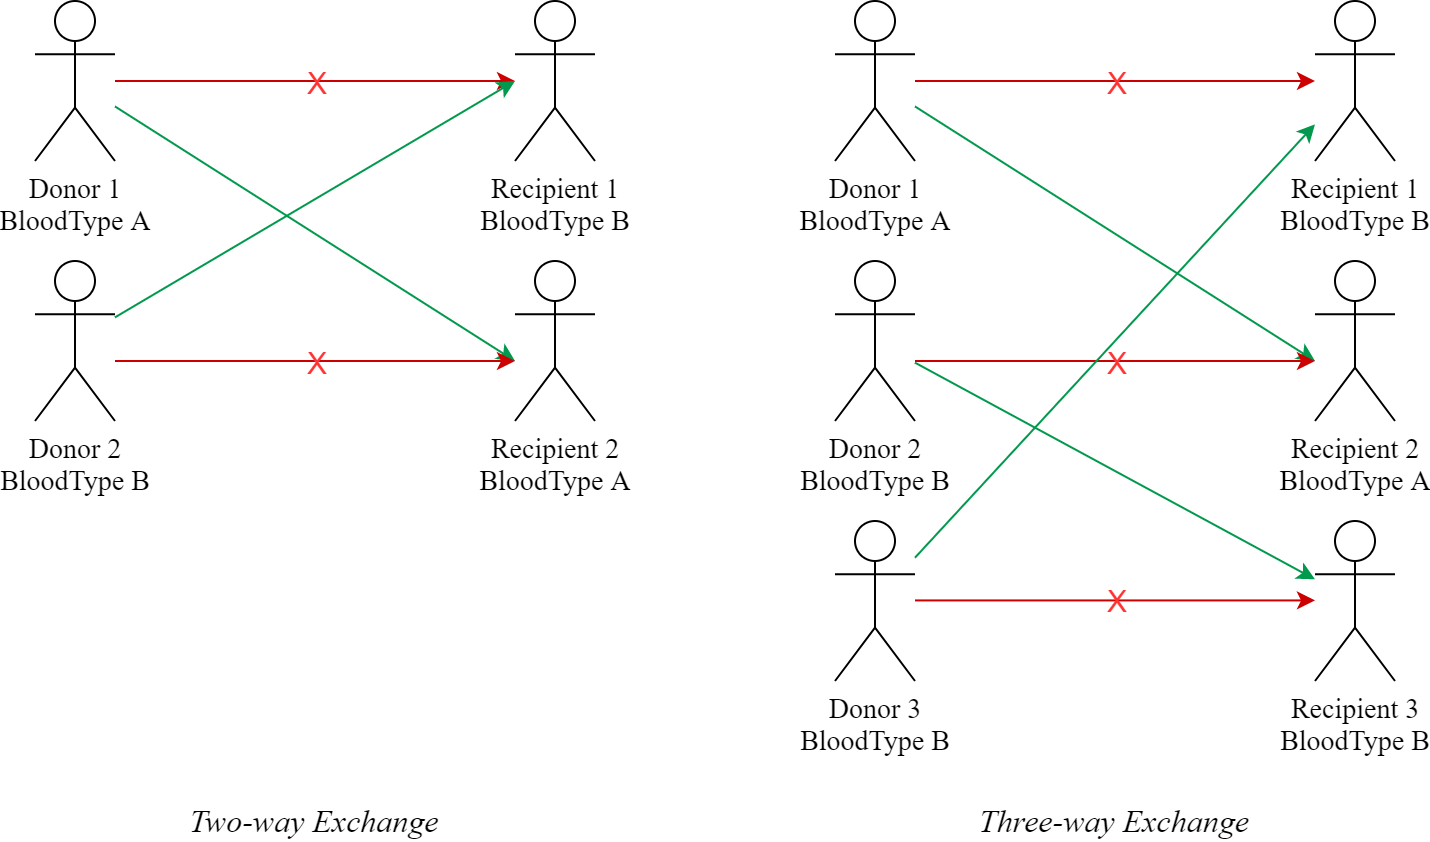
\includegraphics[width=0.5\textwidth]{images/kidney-exchange.png}
    \caption{Pertukaran dua arah(kiri) dan tiga arah(kanan) pada Program Pertukaran Ginjal}
\end{figure}

Karena banyaknya pasangan ketidakcocokan, rumah sakit-rumah sakit tidak dapat secara mudah mendapatkan solusi pencocokan
yang optimal untuk sekumpulan pasangan-pasangna ketidakcocokan. Dibutuhkan algoritma untuk mencarikan pemetaan kecocokan.
Salah satu algoritma yang diketahui untuk menyelesaikan permasalahan ini adalah \textit{Edmond's Algorithm} \cite{raja}.
Pada \textit{Edmond's Algorithm}, kumpulan pasangan ketidakcocokan direpresentasikan dengan suatu graf dengan setiap simpul
yang adalah pasangan ketidakcocokan dan sisi yang merupakan arah pencocokan antar-pasangan yang mungkin. Algoritma ini berfokus
untuk mencarikan kecocokan terlebih dahulu untuk pasangan-pasangan dengan prioritas tinggi sehingga pasien-pasien yang lebih
membutuhkan transplantasi dapat mendapatkan pertukaran terlebih dahulu. Algoritma lain pada lingkup kerja ini adalah algoritma
\textit{First Accept Heuristic Match} \cite{raja} yang menggunakan heuristik dimana pasangan yang registrasi lebih dulu akan
mendapatkan kecocokan terlebih dahulu.

Algoritma-algoritma ini dinamakan algoritma pencarian pemetaan kecocokan. Bagus atau tidaknya algoritma-algoritma ini diukur
menggunakan metrik performa Efisiensi Pencocokan dan Waktu Eksekusi Algoritma \cite{tullis}. Efisiensi pencocokan merepresentasikan
berapa banyaknya pasangan yang mendapatkan kecocokan dari semua pasangan yang ada, ditulis dalam bentuk persentase. Waktu Eksekusi
Algoritma adalah metrik yang mengukur seberapa lama waktu jalannya algoritma dimulai dari \textit{input} masuk hingga \textit{output}
keluar, diukur dalam milisekon (ms). Algoritma pencarian pemetaan kecocokan terbaik merupakan algoritma yang mampu menghasilkan
efisiensi pencocokan yang tinggi dalam waktu eksekusi yang singkat, yang berarti lebih banyak pasien yang lebih dapat terselamatkan
secepat mungkin.

Meskipun \textit{Edmond's Algorithm} dan \textit{First Accept Heuristic Match} sudah ada, algoritma-algoritma
tersebut hanya dapat mengembalikan pertukaran dua arah. Hal ini merupakan suatu batasan karena algoritma-algoritma
ini menutup kemungkinan dicarikannya solusi dengan pertukaran tiga arah atau lebih.

\section{Metodologi}
From the existing algorithms problems addressed in the previous section, match map searching algorithms that can find
\textit{N}-way exchanges from incompatible pairs pool are needed. By modifying existing algorithms and the used data
structure, new algorithms can be created.

\subsection{Compatibility Graph}
Before creating new algorithms, incompatibility pairs pool data structure needs to be redefined. Compatibility Graph
used in Edmond's Algorithm is an undirected graph \cite{raja}, meaning that every edge connecting two vertices represent a bidirectional
relationship between the aforementioned two vertices, making the returned exchanges to be edges, closing up possibility
of three-way exchanges or more. If the algorithm is modified to use cycle detection instead of edge detection, Edmond's
Algorithm can already be used to return \textit{N}-way exchanges.
As seen in Fig. 2, using cycle detection yields a result with three-way exchange instead of the two-way exchange result
returned by edge detection, resulting in a higher matching efficiency using the same compatibility graph. 

\begin{figure}[h]
    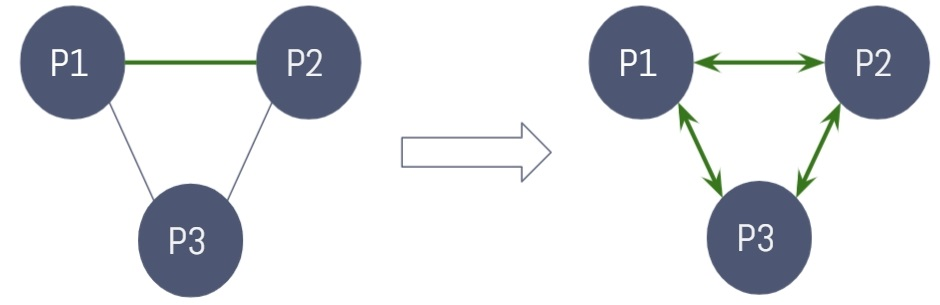
\includegraphics[width=0.5\textwidth]{images/edge-vs-cycle-detection.jpg}
    \caption{Edge Detection(left) vs. Cycle Detection(right) in Compatibility Graph}
\end{figure}

\subsection{Cycle Detection for Directed Graph}
As stated in the previous subsection, edge detection used in existing algorithms needs to be converted to cycle detection.
However, changing edge detection to cycle detection is not enough. The cycles returned from the graph are all bidirectional
cycles. If the compatibility graph is converted into a directed graph instead of undirected, unidirectional cycles can also be
returned, further increasing the number of cycles, therefore increasing the matching efficiency.
Directed graph is a data structure consisting a set of vertices that are connected via edges, where each edge has a one-way
direction that shows the direction of movement from one vertex to another \cite{sedgewick}.
Cycle detection for directed graph is used to find the existence of a one-way path in a graph that starts and finishes
at the same vertex \cite{mehta}.

The cycle detection algorithm being used here is a little bit different from the usual cycle detection algorithm that detects
whether a graph has a cycle or not, instead this algorithm collects and returns all possible cycle in a graph in a list.
Each cycle in this list is a possible exchange that can be excecuted. The length of the cycle represents the \textit{N} in
\textit{N}-way exchange (e.g., a cycle with the length of 3 represents a three-way exchange).
These modification is performed with the hope that the amount of cycles being detected will
increase and therefore increasing matching efficiency and saving more patients.

\subsection{\textit{N}-way Match Map Searching Algorithms}
With directed graph as compatibility graph and using cycle detection algorithm, \textit{N}-way match map searching algorithms
can be created. This algorithms receive the list of cycles returned from cycle detection and returned a reduced list of cycles
called match mapping. The reduction mentioned is done because each pairs in compatibility graph can exist in more than one cycles
in list of cycle, creating a many-to-many relationship among the pairs. This is obviously impossible as every pair can only donate
and receive exactly one kidney. The reduction is done to change this many-to-many relationship to be a one-to-one relationship. This
reduction usually leaves some pairs to be not matched at all, therefore matching efficiency is used as a performance metric to
measure how many pairs can get matched out of the full incompatible pairs pool.  

\subsubsection{First Accept Searching Algorithm}
The first \textit{N}-way match map searching algorithm is first accept searching algorithm which is inspired by first accept
heuristic match algorithm. The first-accept approach being used in this algorithm is to to use the first cycles in cycles list
returned from cycle detection algorithm. This algorithm ensures that no pair gets matched twice or more by deleting cycles that
contains pairs that have been matched earlier.

This algorithm uses two parameters. The first parameter is the number of \textit{N}, knowing that this algororithm is an \textit{N}-way
algorithm. The second parameter is the method to use \textit{N}. The number of \textit{N} can be used as a maximum or exact way of exchanges.
When the maximum method is used, the algorithm will search for cycles that represents two-to-\textit{N}-way exchanges. Meanwhile when exact
method is used, the algorithm will search for cycles that have an exact length of \textit{N}.  

\subsubsection{Priority-based Searching Algorithm}
The second \textit{N}-way match map searching algorithm is priority-based searching algorithm which is inspired by Edmond's
algorithm. This algorithm works similarly with First Accept Searching Algorithm, but each cycle is given a priority value so
that exchanges with highest priority can be returned first compared to the others.

This algorothm uses three parameters. The first two are the same parameter used in First Accept Searching Algortihm, number of \textit{N}
and the method to use \textit{N}. The third parameter is priority assignment method. There are two methods to measure priority of every cycles.
The first assignment method is the greedy method. This method assigns higher priority for longer cycles, indirectly affecting the algorithm
to return more of the longer cycles with the hope that it can increase the matching efficiency.
The second assignment method is the infrequent method. This method assigns higher priority for cycles with infrequent pairs. In implementation,
infrequent pairs are indicated as vertices that are connected with a low number of edges, meaning that the pairs can only be matched with a low
number of other incompatible pairs.

\section{Experiment and Analysis}
Before experiment is performed, Edmond's Algorithm is also implemented as a baseline algorithm so comparisons can be made against
an existing algorithm. The data being used in this experiment can be found in this link: \url{https://rdm.inesctec.pt/dataset/ii-2020-001}
while the source code of the implementation and the experiment can be found in this link: \url{https://github.com/Mingtaros/Kidney-Exchange-Match-Mapping-System}.
The purpose of these experiments and evaluations are to find the algorithm and parameter combinations which can produce the best
performance results based on pre-defined metrics. In addition, through the experiments, it can be concluded which \textit{N}-way
algorithm and parameter combinations are able to outperform the baseline, Edmond's Algorithm. Based on the pre-defined metrics,
there will be comparison for Execution Time and Matching Efficiency for each algorithm.

\subsection{Execution Time Comparison}
\subsubsection{Execution Time Comparison for Different Algorithm Combinations}
For this experiment, each algorithm is used for 3000 incompatible pairs divided into 30 groups of 100. A group is called a seed. Each
algorithm will be fitted with the same dataset group 50 times for every group. As seen in Figure \ref{exctimealgo}, each data point in the boxplot
is used to show the average execution time from the 50 executions for every dataset group, in one Y coordinate, there are 30 data
points, each one for one data group. 

\begin{figure}[h]
    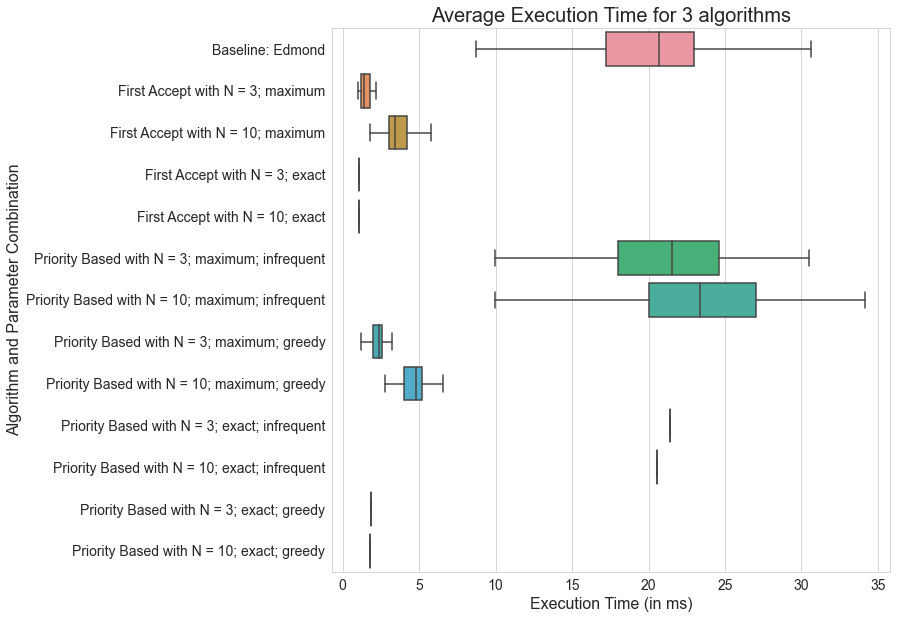
\includegraphics[width=0.5\textwidth]{images/average_execution_time_for_3_algorithms.png}
    \caption{Average Execution Time for 3 Algorithms}
    \label{exctimealgo}
\end{figure}

As seen from the boxplot, Edmond's Algorithm and Priority-based with infrequent method of priority assignment are the slowest
algorithms. However, given that each and every algorithm does not have a significant difference in execution time, the execution
time difference can be ignored.

\subsubsection{Execution Time Comparison for Different Data Sizes}
This experiment is conducted to show the effect of data size to execution time of the match map searching algorithms. For this
experiment, the recorded execution time is the average execution time for each algorithm using data size of  100, 200, 300, 400,
500, 1000, 2000, as well as 3000 incompatible pairs. Each data point is the average of algorithm execution time that has been
executed 10 times for each algorithm for each data size.

\begin{figure}[h]
    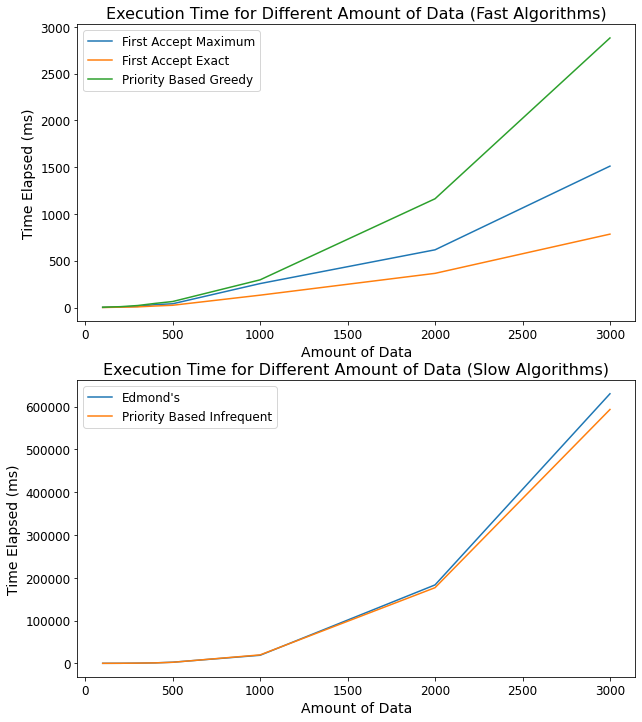
\includegraphics[width=0.5\textwidth]{images/execution_time_for_different_amount_of_data.png}
    \caption{Execution Time for Different Amount of Data}
    \label{exctimedata}
\end{figure}

As seen in Figure \ref{exctimedata}, there are two plots, each one representing a group of fast algorithms and a group of slow algorithms.
From the upper figure, even with 3000 incompatible pairs, the maximum algorithm runtime is around 3000 milliseconds. Meanwhile,
from the lower figure, both of the algorithms can reach 600000 milliseconds (10 minutes) to process 3000 pairs. From the
overall line plot, it can be concluded that the relation of data size and execution time is a form of polynomial function, not linear.

\subsection{Overall Matching Efficiency Comparison for Different Algorithms}
The final experiment is conducted to show which algorithm-parameter combination is the best one in producing high matching efficiency.
In this experiment, each combination is used for every data seed. To ease up the comparison, in Figure \ref{matcheffratio}, ratio of improvement is used
in comparison to Edmond's Algorithm as a baseline shown as a horizontal line in the figure. Every data point is a matching efficiency
multiplier of the matching efficiency obtained when Edmond's Algorithm is used.

\begin{figure}[h]
    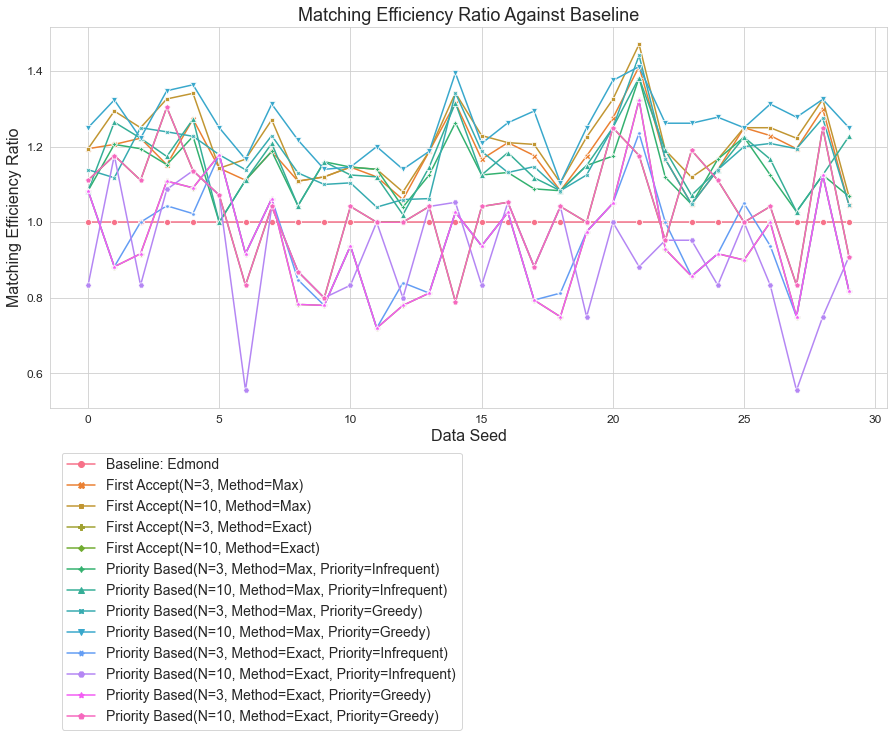
\includegraphics[width=0.5\textwidth]{images/matching_efficiency_ratio_against_baseline.png}
    \caption{Matching Efficiency Ratio of \textit{N}-way Algorithms against Baseline}
    \label{matcheffratio}
\end{figure}

To simplify the figure, Table \ref{tab2} is used to store average matching efficiency improvement ratio in compared to baseline. The average used
in the table is the average improvement ratio of an algorithm in comparison to baseline for all data seeds.

\begin{table}[htbp]
    \caption{Average Matching Efficiency Ratio of \textit{N}-way Algorithms compared to Baseline}
    \begin{center}
    \def\arraystretch{1.5}
    \begin{tabular}{|c|c|}
    \hline
    \cellcolor{tableheader}&\cellcolor{tableheader}\textbf{Average} \\
    \cellcolor{tableheader}\textbf{Algorithm}&\cellcolor{tableheader}\textbf{Improvement}\\
    \cellcolor{tableheader}&\cellcolor{tableheader}\textbf{Ratio}\\
    \hline
    Baseline: Edmond's Algorithm&1.0 \\
    \hline
    First Accept(N=3, Method=Max)&\cellcolor{moreratio}1.18 \\
    \hline
    First Accept(N=10, Method=Max)&\cellcolor{moreratio}1.22 \\
    \hline
    First Accept(N=3, Method=Exact)&\cellcolor{lessratio}0.94 \\
    \hline
    First Accept(N=10, Method=Exact)&\cellcolor{moreratio}1.04 \\
    \hline
    Priority Based(N=3, Method=Max, Priority=Greedy)&\cellcolor{moreratio}1.17 \\
    \hline
    Priority Based(N=10, Method=Max, Priority=Greedy)&\cellcolor{moreratio}1.26 \\
    \hline
    Priority Based(N=3, Method=Max, Priority=Infrequent)&\cellcolor{moreratio}1.14 \\
    \hline
    Priority Based(N=10, Method=Max, Priority=Infrequent)&\cellcolor{moreratio}1.16 \\
    \hline
    Priority Based(N=3, Method=Exact, Priority=Greedy)&\cellcolor{lessratio}0.94 \\
    \hline
    Priority Based(N=10, Method=Exact, Priority=Greedy)&\cellcolor{moreratio}1.04 \\
    \hline
    Priority Based(N=3, Method=Exact, Priority=Infrequent)&\cellcolor{lessratio}0.95 \\
    \hline
    Priority Based(N=10, Method=Exact, Priority=Infrequent)&\cellcolor{lessratio}0.91 \\
    \hline
    \end{tabular}
    \label{tab2}
    \end{center}
\end{table}

As can be seen from Table \ref{tab2}, most of \textit{N}-way match map searching algorithm produces higher matching efficiency in
comparison to the baseline, Edmond's Algorithm. However, some algorithms, using the exact method of using \textit{N} parameter,
have worse results compared to baseline. The average matching efficiency of the \textit{N}-way match map searching
algorithms is 7.75\% higher than the baseline algorithm. The higher matching efficiency improvement is obtained when First Accept
Searching algorithm is used when \textit{N} is 10, maximum method of using \textit{N}, with data seed 21, where the improvement
against baseline is 47.06\%.

While \textit{N}-way match map searching algorithms may produce better results, it is worth noting that with \textit{N}-way exchanges
being produced by algorithm may be harder to execute in hospitals since the kidney exchanges have to be operated in the same time. The
implication is that exchanges with lower number of ways are easier to conduct as less hospital resources are needed to conduct the operation.
Therefore, there needs to be an algorithm comparison regarding the average and the maximum exchanges length of the cycles in the match map.
In this experiment, every algorithm and parameter combinations are being tested for 30 data seeds with each containing 100 incompatible pairs. 

\begin{figure}[h]
   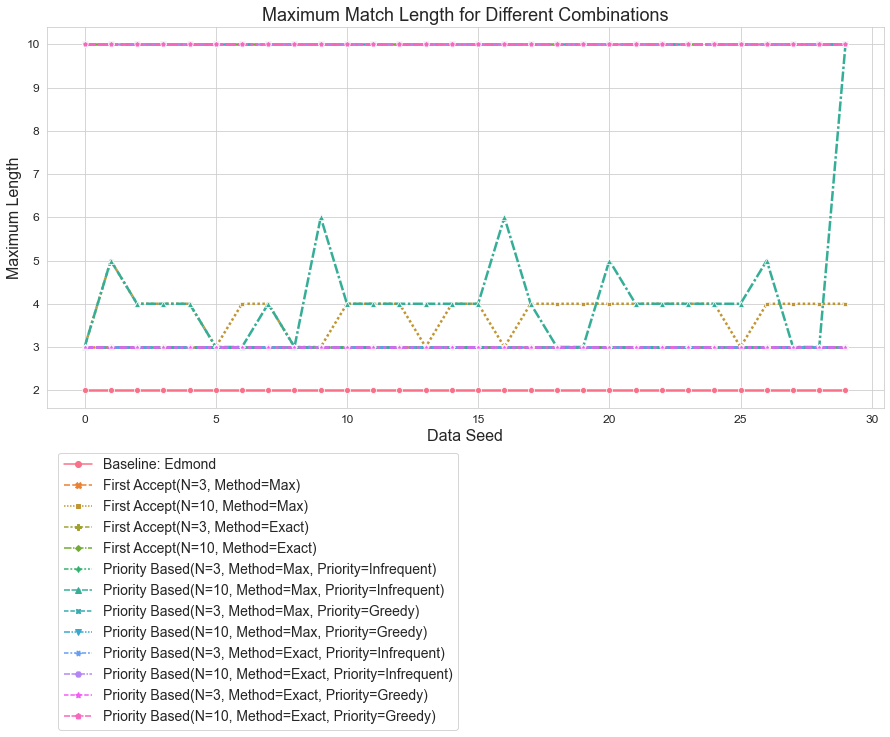
\includegraphics[width=0.5\textwidth]{images/maximum_match_length_for_different_combinations.png}
   \caption{Maximum Match Length for Different Algorithm Combinations}
   \label{figuremaxlength}
\end{figure}

From what can be seen in Figure \ref{figuremaxlength}, Edmond's Algorithm and algorithms with \textit{N} usage method parameter assigned to exact, produced the maximum
length of \textit{N} as the cycles in the produced match map is all of the same length that is \textit{N}.
The more interesting result is that although the parameter \textit{N} is 10, as can be seen with the green and the yellow line, the maximum length is
is not that close to 10. 

\begin{figure}[h]
    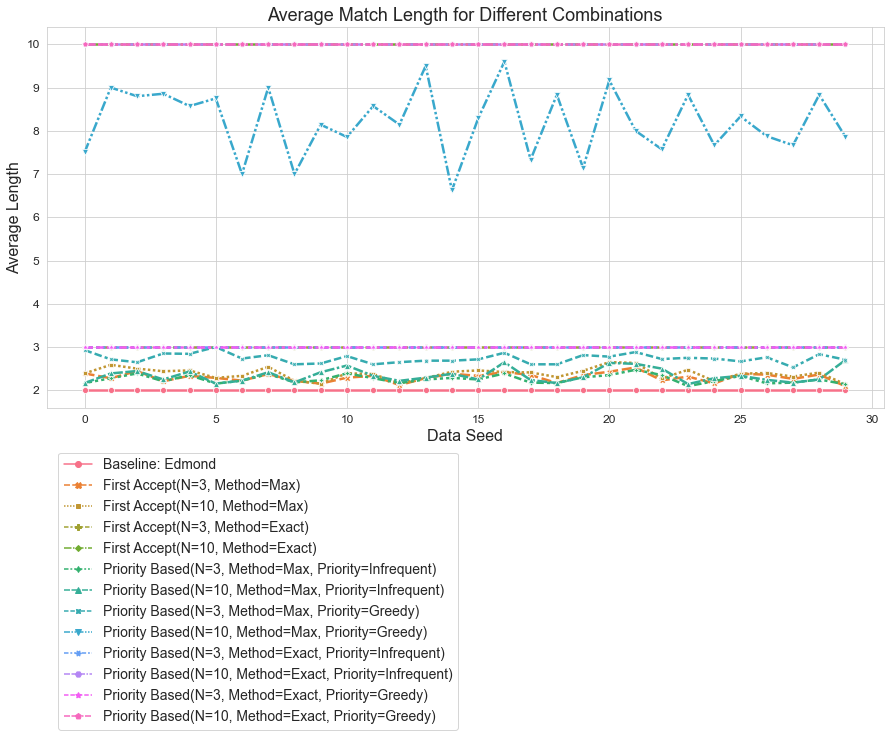
\includegraphics[width=0.5\textwidth]{images/average_match_length_for_different_combinations.png}
    \caption{Average Match Length for Different Algorithm Combinations}
    \label{figureavglength}
\end{figure}

Similar to what can be seen in Figure \ref{figuremaxlength}, in Figure \ref{figureavglength}, Edmond's Algorithm and algorithms with
\textit{N} usage method parameter assigned to exact, produced the average length of \textit{N} as the cycles in the produced match map is all
of the same length that is \textit{N}. Generally, almost every algorithm that uses maximum method of \textit{N} usage produces cycles with the
average length of around 2 to 3, with Priority-based Searching algorithm with N=10, Method=Max, and Priority=Greedy, having an averagely high
average length of exchanges.

\section{Conclusion}
This paper shows that it is a viable option to use \textit{N}-way match map searching algorithms instead of the usual two-way
algorithms such as Edmond's Algorithm for Kidney Paired Donation, with \textit{N}-way algorithms producing better matching efficiency
and competitive execution time in comparison to the baseline, Edmond's Algorithm provided the same dataset. Generally speaking,
the usage of \textit{N}-way algorithms increases matching efficiency by 7.75\%.

With the provided data, First Accept Searching algorithm have a more consistent performance in general compared to Priority-based Searching
algorithm. However, with Priority-based Searching algorithm, the matching efficiency improvement is generally higher with the exception of
when exact method to utilize \textit{N} is being used instead of the maximum method. However, it is worth noting that priority-based searching
algorithm may produce high matching efficiency with the compromise of high average matching length if greedy priority assignment method is being
used. Therefore it can be concluded that First Accept Searching algorithm is the most ideal \textit{N}-way match map searching algorithm to use
in Kidney Exchange Program. 

\section{Related Work}
The idea of the solution, the existing algorithms, and the performance metrics being used as a performance measure are all obtained from
the main reference paper, Web Based Decision Support System for Kidney Exchange by Samy Raja, Prasanna Devi S., and Suryaprakasa Rao K. in
International Journal of Computer Applications \cite{raja}. In that paper, two-way match map searching algorithms are being used to tackle
the problem of the humanely-impossible task of searching the most optimal match map out of an incompatible pairs pool, which becomes the baseline
and the reference of the newer algorithms being implemented in this paper.

\begin{thebibliography}{00}
\bibitem{roth2005} Roth, A. E., Sonmez, T., Unver, M. U. (2005). Kidney Exchange. Quarterly Journal of Economics, 32.
\bibitem{wiradarma} Wiradarma, K. (2016, February 3). Transplantasi Ginjal di Indonesia: Pencapaian dan Hambatannya. Retrieved from klikdokter.com: https://www.klikdokter.com/info-sehat/read/2697086/transplantasi-ginjal-di-indonesia-pencapaian-dan-hambatannya
\bibitem{roth2006} Roth, A. E., Sonmez, T., Unver, M. U., Delmonico, F. L., Saidman, S. L. (2006, September 18). Utilizing List Exchange and Nondirected Donation through ‘Chain’ Paired Kidney Donations. Retrieved from onlinelibrary.wiley.com: https://onlinelibrary.wiley.com/doi/full/10.1111/j.1600-6143.2006.01515.x
\bibitem{adrian} Adrian, K. (2020, May 17). Berbagai Persiapan Donor Ginjal yang Perlu Anda Ketahui. Retrieved from alodokter.com: https://www.alodokter.com/hal-hal-yang-harus-diperhatikan-sebelum-melakukan-donor-ginjal
\bibitem{raja} Raja, S., S., P. D., K., S. R. (2011). Web Based Decision Support System for Kidney. International Journal of Computer Applications (0975 – 8887), 9.
\bibitem{charge} Chargé, S., Hodgkinson, K. (2017, January). Blood: the basics. Retrieved from profedu.blood.ca/: https://profedu.blood.ca/en/transfusion/publications/blood-basics.
\bibitem{aprilano} Aprilano, W. D. (2021, January 20). Teknik Transplantasi Ginjal. Retrieved from alomedika.com: https://www.alomedika.com/tindakan-medis/transplantasi/transplantasi-ginjal/teknik
\bibitem{nguyen} Nguyen, H. D., Williams, R. L., Wong, G., Lim, W. H. (2013, February 13). The Evolution of HLA-Matching in Kidney Transplantation. Retrieved from intechopen.com: https://www.intechopen.com/books/current-issues-and-future-direction-in-kidney-transplantation/the-evolution-of-hla-matching-in-kidney-transplantation
\bibitem{tullis} Tullis, T., Albert, B. (2013, June 3). Performance Metrics. Retrieved from sciencedirect.com: https://www.sciencedirect.com/science/article/pii/B9780124157811000042
\bibitem{sedgewick} Sedgewick, R., Wayne, K. (2020). Directed Graphs. In R. Sedgewick, K. Wayne, Algorithms, 4th Edition (p. 955). New Jersey: Princeton University.
\bibitem{mehta} Mehta, D. (2020, May 27). Detect Cycle in a Directed Graph. Retrieved from geeksforgeeks.org: https://www.geeksforgeeks.org/detect-cycle-in-a-graph/
\end{thebibliography}

\end{document}
